% =====================================================================
%  Proposed methodology, end to end: two datasets in, one shared trunk,
%  two task heads, two sets of metrics.
%
%  Deliberately plain: rounded boxes and arrows only, five bands, ten
%  boxes, no title or caption -- the figure alone, so the caption can
%  live in the slide or the paper. The trunk is ONE box on purpose;
%  what is inside it is the job of fig_tomanet_c / fig_tomanet_d /
%  fig_tomalayer_usage. Colours come from the shared palette so a
%  module keeps the same colour in every figure.
%
%  Layout rules that keep it clean:
%    - every band is a panel with its number inside the top left;
%    - all routing happens in the gaps between panels, so no connector
%      ever crosses a label;
%    - every arrow ends on a node anchor (.north / .south), never on a
%      bare coordinate, so nothing floats short of its box.
%
%  Build:
%    pdflatex -interaction=nonstopmode fig_proposed_methodology.tex
%    pdftoppm -jpeg -r 300 -singlefile fig_proposed_methodology.pdf \
%             fig_proposed_methodology_300dpi
% =====================================================================
\documentclass[border=14pt, tikz]{standalone}
\usepackage[T1]{fontenc}
\usepackage{newtxtext,newtxmath}   % Times New Roman metrics
\usetikzlibrary{positioning,calc,backgrounds,arrows.meta}
% =====================================================================
%  tomanet_palette.tex -- one colour per architectural role, shared by
%  fig_tomanet_c.tex and fig_tomanet_d.tex so a shared module (the stem
%  and backbone) keeps the exact same colour in both figures. That
%  visual identity IS the point: TomaNet-C and TomaNet-D use a
%  byte-identical trunk (layers 0-8) and only the colours after the
%  trunk change.
% =====================================================================
\definecolor{tStem}   {RGB}{243,203,150}  % stem convs             sand
\definecolor{tStemP}  {RGB}{253,240,222}  % stem panel
\definecolor{tTrunk}  {RGB}{150,196,140}  % TomaLayer stages        leaf green
\definecolor{tTrunkP} {RGB}{232,244,227}  % trunk panel
\definecolor{tBlkA}   {RGB}{120,175,190}  % RepPConv / spatial      teal
\definecolor{tBlkB}   {RGB}{150,150,200}  % CoordAtt                periwinkle
\definecolor{tNeck}   {RGB}{ 90,110,175}  % TomaLayer, neck (e=1.0) deep slate blue
\definecolor{tNeckP}  {RGB}{231,236,247}  % neck panel
\definecolor{tStruct} {RGB}{200,200,200}  % structural ops: upsample / concat -- not a learned layer, so deliberately neutral grey
\definecolor{tHeadC}  {RGB}{210,110,90}   % classify head           tomato red
\definecolor{tHeadCP} {RGB}{250,231,225}  % classify head panel
\definecolor{tHeadD}  {RGB}{210,110,90}   % detect heads            tomato red (same family: both are "the answer")
\definecolor{tHeadDP} {RGB}{250,231,225}  % detect head panel
\definecolor{tLine}   {RGB}{ 90,100,95}   % connector
\definecolor{tRule}   {RGB}{200,206,200}  % separators

% ---- PlotNeuralNet 3D-tile band colours (darker shade of each block's
% own hue, used for RightBandedBox's second face -- e.g. "the BN+act
% half" or "the attention half" of a two-part operation) -------------
\colorlet{tStemBand}  {tStem!60!black}
\colorlet{tTrunkBand} {tTrunk!60!black}
\colorlet{tNeckBand}  {tNeck!60!black}
\colorlet{tHeadCBand} {tHeadC!60!black}
\colorlet{tHeadDBand} {tHeadD!60!black}
\colorlet{tBlkABand}  {tBlkA!60!black}
\colorlet{tBlkBBand}  {tBlkB!60!black}
\definecolor{tBlkSum} {RGB}{190,140,150}  % residual / concat ball    dusty rose


\begin{document}
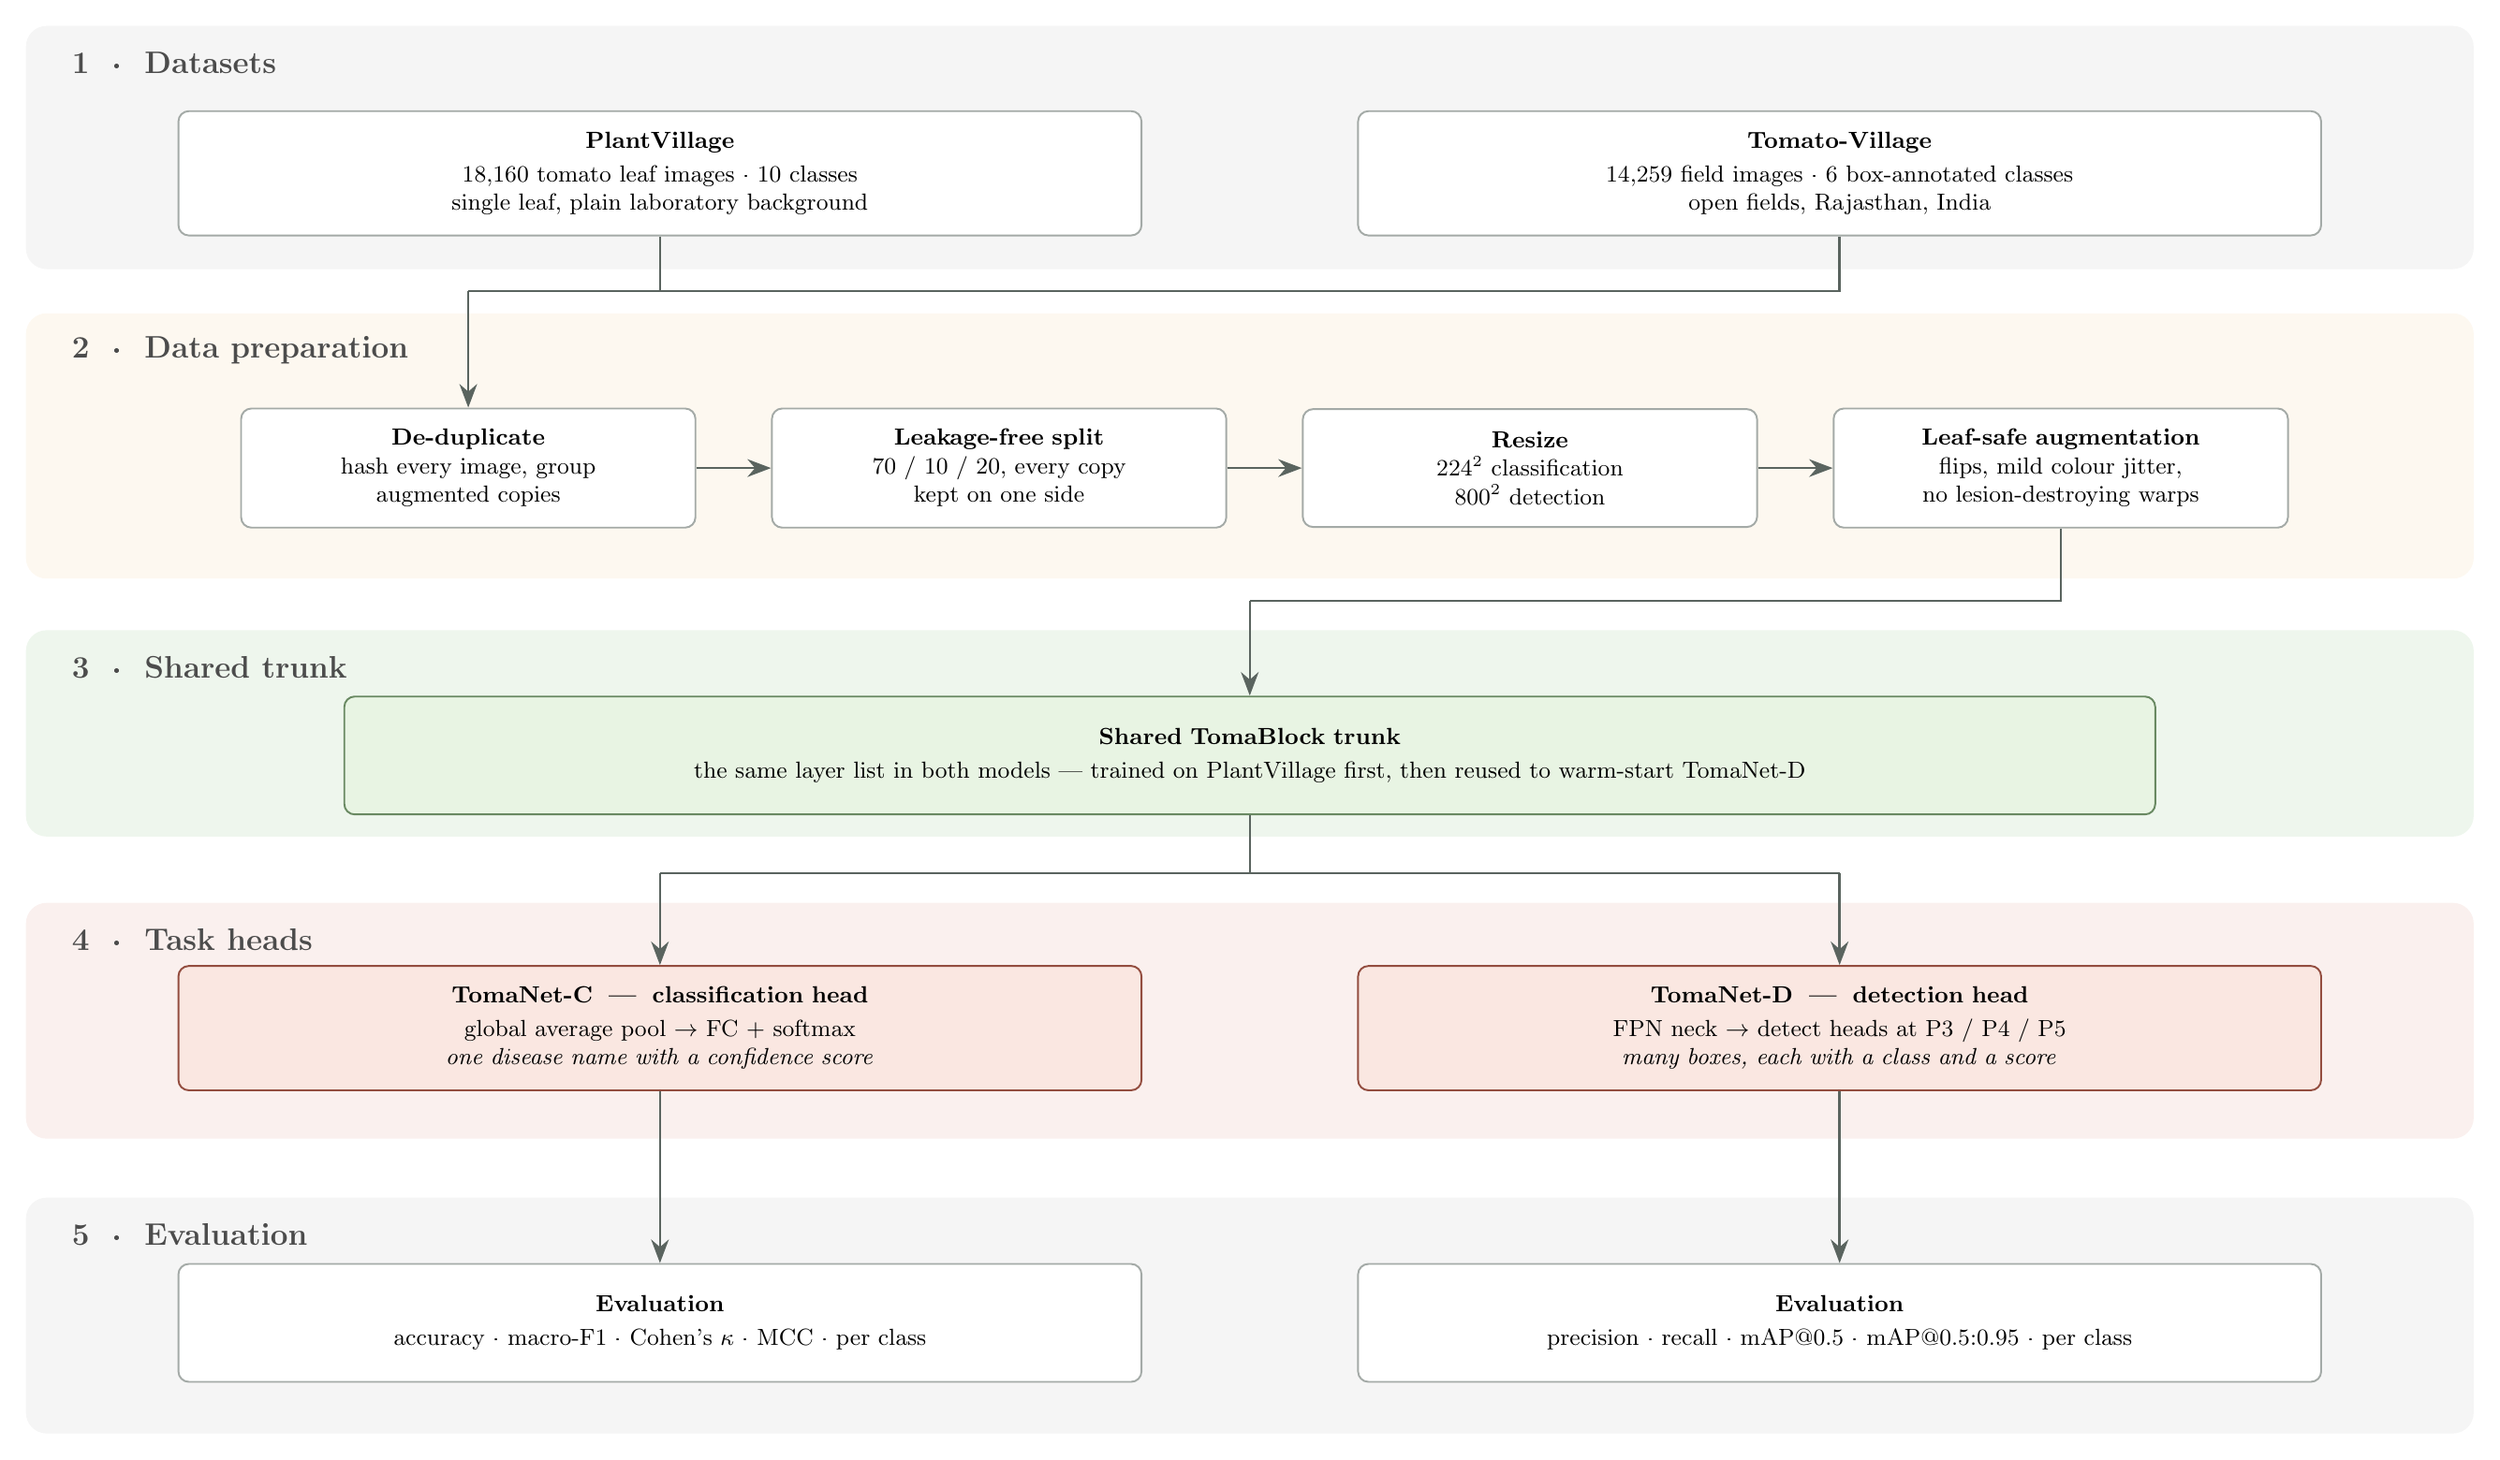
\begin{tikzpicture}

% ---------------------------------------------------------------- styles
\tikzset{
  blk/.style   = {rounded corners=4pt, draw=tLine!55, line width=0.7pt,
                  fill=white, align=center, inner sep=8pt,
                  minimum height=1.6cm, font=\small},
  trunk/.style = {blk, fill=tTrunkP, draw=tTrunk!70!black},
  headc/.style = {blk, fill=tHeadCP, draw=tHeadC!70!black},
  headd/.style = {blk, fill=tHeadDP, draw=tHeadD!70!black},
  band/.style  = {font=\large\bfseries, anchor=west, text=black!70},
  line/.style  = {draw=tLine, line width=0.9pt},
  arr/.style   = {line, -{Stealth[length=3.2mm,width=2.4mm]}},
}

% ================================================================ 1 data
\node[blk, text width=12.5cm] (pv) at (9,-2.4)
  {\textbf{PlantVillage}\\[2pt]
   18,160 tomato leaf images \textperiodcentered\ 10 classes\\
   single leaf, plain laboratory background};
\node[blk, text width=12.5cm] (tv) at (25,-2.4)
  {\textbf{Tomato-Village}\\[2pt]
   14,259 field images \textperiodcentered\ 6 box-annotated classes\\
   open fields, Rajasthan, India};

% ========================================================= 2 preparation
\node[blk, text width=5.6cm] (p1) at (6.4,-6.4)
  {\textbf{De-duplicate}\\ hash every image, group\\ augmented copies};
\node[blk, text width=5.6cm] (p2) at (13.6,-6.4)
  {\textbf{Leakage-free split}\\ 70 / 10 / 20, every copy\\ kept on one side};
\node[blk, text width=5.6cm] (p3) at (20.8,-6.4)
  {\textbf{Resize}\\ $224^2$ classification\\ $800^2$ detection};
\node[blk, text width=5.6cm] (p4) at (28.0,-6.4)
  {\textbf{Leaf-safe augmentation}\\ flips, mild colour jitter,\\ no lesion-destroying warps};
\draw[arr] (p1) -- (p2);
\draw[arr] (p2) -- (p3);
\draw[arr] (p3) -- (p4);

% =========================================================== 3 the trunk
\node[trunk, text width=24cm] (tr) at (17,-10.3)
  {\textbf{Shared TomaBlock trunk}\\[2pt]
   the same layer list in both models --- trained on PlantVillage first,
   then reused to warm-start TomaNet-D};

% =========================================================== 4 the heads
\node[headc, text width=12.5cm] (hc) at (9,-14.0)
  {\textbf{TomaNet-C \ \textemdash\ \ classification head}\\[2pt]
   global average pool $\rightarrow$ FC $+$ softmax\\
   \emph{one disease name with a confidence score}};
\node[headd, text width=12.5cm] (hd) at (25,-14.0)
  {\textbf{TomaNet-D \ \textemdash\ \ detection head}\\[2pt]
   FPN neck $\rightarrow$ detect heads at P3 / P4 / P5\\
   \emph{many boxes, each with a class and a score}};

% ============================================================ 5 metrics
\node[blk, text width=12.5cm] (ec) at (9,-18.0)
  {\textbf{Evaluation}\\[2pt]
   accuracy \textperiodcentered\ macro-F1 \textperiodcentered\
   Cohen's $\kappa$ \textperiodcentered\ MCC \textperiodcentered\ per class};
\node[blk, text width=12.5cm] (ed) at (25,-18.0)
  {\textbf{Evaluation}\\[2pt]
   precision \textperiodcentered\ recall \textperiodcentered\ mAP@0.5
   \textperiodcentered\ mAP@0.5:0.95 \textperiodcentered\ per class};

% ------------------------------------------------- routing, in the gaps
% both datasets feed the same four preparation steps
\draw[line] (pv.south) |- (6.4,-4.0);
\draw[line] (tv.south) |- (6.4,-4.0);
\draw[arr]  (6.4,-4.0) -- (p1.north);
% prepared data goes into the trunk
\draw[line] (p4.south) -- (28.0,-8.2) -- (17.0,-8.2);
\draw[arr]  (17.0,-8.2) -- (tr.north);
% the trunk feeds both heads
\draw[line] (tr.south) -- (17.0,-11.9);
\draw[line] (9.0,-11.9) -- (25.0,-11.9);
\draw[arr]  (9.0,-11.9)  -- (hc.north);
\draw[arr]  (25.0,-11.9) -- (hd.north);
% heads to metrics
\draw[arr] (hc.south) -- (ec.north);
\draw[arr] (hd.south) -- (ed.north);

% ---------------------------------------------------------------- panels
\begin{scope}[on background layer]
  \fill[black!4,   rounded corners=8pt] (0.4, -0.4)  rectangle (33.6, -3.7);
  \fill[tStem!14,  rounded corners=8pt] (0.4, -4.3)  rectangle (33.6, -7.9);
  \fill[tTrunk!16, rounded corners=8pt] (0.4, -8.6)  rectangle (33.6,-11.4);
  \fill[tHeadC!10, rounded corners=8pt] (0.4,-12.3)  rectangle (33.6,-15.5);
  \fill[black!4,   rounded corners=8pt] (0.4,-16.3)  rectangle (33.6,-19.5);
\end{scope}

\node[band] at (0.9, -0.9)  {1 \ \textperiodcentered\ \ Datasets};
\node[band] at (0.9, -4.8)  {2 \ \textperiodcentered\ \ Data preparation};
\node[band] at (0.9, -9.1)  {3 \ \textperiodcentered\ \ Shared trunk};
\node[band] at (0.9,-12.8)  {4 \ \textperiodcentered\ \ Task heads};
\node[band] at (0.9,-16.8)  {5 \ \textperiodcentered\ \ Evaluation};

\end{tikzpicture}
\end{document}
